\subsection{Требования к проектируемому программному средству}
\label{sec:analysis:specification}

По результатам изучения предметной области, анализа литературных источников и обзора существующих систем-аналогов
сформулируем требования к проектируемому программному средству.
\pagebreak

\subsubsection{} Назначение проекта
\label{sec:analysis:specification:purpose}

Назначением проекта является разработка программного средства, обеспечивающего отслеживание
активных вакансии в компании, текущую занятость сотрудников на проектах, их способности, а также автоматическая генерация
на основе полученных данных резюме сотрудника для дальнейшего использования в отделе маркетинга и продаж.

\subsubsection{} Основные функции
\label{sec:analysis:specification:functions}

Программное средство должно поддерживать следующие основные фун\-к\-ции:

\begin{itemize}
	\item регистрация и аутентификация;
	\item возможность приглашения пользователей;
	\item поддержка системы ролей;
	\item управление проектами организации;
	\item управление отделами организации;
	\item управление должностями;
	\item управление профилями пользователей;
	\item управление вопросами для генерации резюме;
	\item генерация резюме;
	\item возможность проверки резюме другими сотрудниками организации;
	\item уведомление сотрудников о необходимости проверки резюме.
\end{itemize}

\subsubsection{} Требования к входным данным
\label{sec:analysis:specification:inputs}

Входные данные для программного средства должны быть представлены в виде вводимого пользователем с помощью клавиатуры
текста и выбора доступных опций пользовательского интерфейса.

Должны быть реализованы проверки вводимых данных на корректность с отображением информации об ошибках в случае их
некорректности.

\subsubsection{} Требования к выходным данным
\label{sec:analysis:specification:outputs}

Выходные данные программного средства должны быть представлены посредством отображения информации с помощью различных
элементов пользовательского интерфейса.

\subsubsection{} Требования к временным характеристикам
\label{sec:analysis:specification:timing}

Производительность программно-аппаратного комплекса должна обеспечивать следующие временные характеристики: время
реакции не запрос пользователя не должно превышать 2 секунд при минимальной скорости соединения 10 МБит/с. Допускается
невыполнение данного требования в случае, когда невозможность обеспечить заявленную производительность обусловлена
объективными внешними причинами.

\subsubsection{} Требования к надежности
\label{sec:analysis:specification:reliability}

Надежное функционирование программы должно быть обеспечено выполнением следующих организационно-технических мероприятий:

\begin{itemize}
	\item организация бесперебойного питания;
	\item выполнение рекомендаций Министерства труда и социальной защиты РБ, изложенных в Постановлении от 23 марта 2011 г. «Об утверждении Норм времени на работы по обслуживанию персональных электронно-вы\-числи\-тельных машин, организационной техники и офисного оборудования»;
	\item выполнение требований ГОСТ 31078-2002 <<Защита информации. Испытания программных средств на наличие компьютерных вирусов>>;
	\item необходимым уровнем квалификации пользователей.
\end{itemize}


Время восстановления после отказа, вызванного сбоем электропитания технических средств (иными внешними факторами),
нефатальным сбоем операционной системы, не должно превышать времени, необходимого на перезагрузку операционной системы
и запуск программы, при условии соблюдения условий эксплуатации технических и программных средств. Время восстановления
после отказа, вызванного неисправностью технических средств, фатальным сбоем операционной системы, не должно
превышать времени, требуемого на устранение неисправностей технических средств и переустановки программных средств.

Отказы программы возможны вследствие некорректных действий пользователя при взаимодействии с операционной системой.
Во избежание возникновения отказов программы по указанной выше причине следует обеспечить работу конечного
пользователя без предоставления ему административных привилегий.

\subsubsection{} Требования к аппаратному обеспечению серверной части
\label{sec:analysis:specification:server_requirments}

ЭВМ, на которой должна функционировать серверная часть программного средства, должна обладать следующими
минимальными характеристиками:

\begin{itemize}
	\item процессор Intel Core i5 с тактовой частотой 2 ГГц;
	\item жесткий диск объемом 100 Гб;
	\item оперативная память 4 Гб;
	\item сетевая карта Ethernet 100 МБит/с.
\end{itemize}

Также для функционирования серверной части требуется установленный Ruby on Rails сервер, который работает на
операционной системе Linux.

\subsubsection{} Требования к аппаратному обеспечению клиентской части
\label{sec:analysis:specification:client_requirments}

Клиентская часть программного средства должна функционировать на ЭВМ со следующими минимальными характеристиками:

\begin{itemize}
	\item процессор Intel Сeleron с тактовой частотой 2 ГГц и более;
	\item оперативная память 4 Гб и более;
	\item возножность выхода в сеть Интернет.
\end{itemize}

Для корректной работы программного средства необходим один из следующих браузеров с соответствующей минимальной версией:

\begin{itemize}
	\item Google Chrome 70;
	\item Opera 58;
	\item Mozilla Firefox 66;
	\item Apple Safari 12.0;
	\item Microsoft Edge 44.
\end{itemize}

\subsubsection{} Выбор технологий программирования
\label{sec:analysis:specification:language}

Язык программирования, на котором будет реализована система, заслуживает большого внимания, так как вы будете
погружены в него с начала конструирования программы до самого конца. Исследования показали, что выбор языка
программирования несколькими способами влияет на производительность труда программистов и качество создаваемого ими
кода. Если язык хорошо знаком программистам, они работают более производительно. Данные, полученные при помощи модели
оценки Cocomo II, показывают, что программисты, использующие язык, с которым они работали три года или более, примерно
на 30\% более продуктивны, чем программисты, обладающие аналогичным опытом, но для которых язык является
новым~\cite{software_cost_estimation}. В более раннем исследовании, проведенном в IBM, было обнаружено, что
программисты, обладающие богатым опытом использования языка программирования, были более чем втрое
производительнее программистов, имеющих минимальный опыт~\cite{method_of_programming_measurement_and_estimation}.

JavaScript ("JS" для краткости) — это полноценный динамический язык программирования, который применяется к HTML
документу, и может обеспечить динамическую интерактивность на веб-сайтах.

JavaScript сам по себе довольно компактный, но очень гибкий. Разработчиками написано большое количество инструментов
поверх основного языка JavaScript, которые разблокируют огромное количество дополнительных функций с очень
небольшим усилием. К ним относятся:

\begin{itemize}
	\item программные интерфейсы приложения (API), встроенные в браузеры, обеспечивающие различные функциональные
	возможности, такие как динамическое создание HTML и установку CSS стилей, захват и манипуляция видеопотоком, работа с
	веб-камерой пользователя или генерация 3D графики;
	\item сторонние API позволяют разработчикам внедрять функциональ\-ность в свои сайты от других разработчиков,
	таких как Twitter или Facebook;
	\item также есть возможность применить к HTML сторонние фреймворки и библиотеки, что позволит ускорить создание
	сайтов и приложений~\cite{javascript_basics}.
\end{itemize}

Выбранный язык программирования является средством для программирования клиентской части приложения.
Поскольку для приложения в любом случае понадобится база данных, то есть два варианта:

\begin{itemize}
	\item осуществлять запросы к БД напрямую с клиентского приложения;
	\item реализовать серверную прослойку между клиентской частью и базой данных.
\end{itemize}

Первый подход крайне небезопасен: очень опасно предоставлять открытый доступ к БД. В это же время, второй способ,
помимо ее сокрытия, предоставляет возможность проверки подлинности и предоставления прав пользователям.
В связи с этим появляется проблема выбора технологий для серверной части. Основным влияющим фактором является
имеющийся опыт команды разработки, в связи с чем была выбрана технология Ruby on Rails и язык программирования Ruby.

Язык программирования Ruby, является кроссплатформенным языком программирования. Ruby -- это тщательно сбалансированный
язык. Его создатель Юкихиро Мацумото, объединил части его любимых языков (Perl, \linebreak Smalltalk, Eiffel, Ada и Lisp) чтобы
сформировать новый язык, в котором парадигма функционального программирования сбалансирована принципами
императивного программирования. 

В Ruby всё -- объект. Для каждой частицы информации или кода могут быть определены собственные свойства и действия.
В объектно-ориентирован\-ном программировании свойства называются переменными объекта, а действия – методами.
Чистейший объектно-ориентированный подход Ruby может быть продемонстрирован парой строк кода, в которых производится
действие над числом.

Во многих языках числа и другие примитивные типы данных не являются объектами. Ruby под влиянием языка Smalltalk
позволяет задать методы и переменные объекта всем типам данных. Это упрощает использование Ruby, так как правила
применимые к объектам -- применимы ко всему Ruby~\cite{ruby}.

Ruby on Rails - фреймворк для веб-разработки, написанный на языке программирования Ruby. Он разработан, чтобы сделать
программирование веб-приложений проще, так как использует ряд допущений о том, что нужно каждому разработчику для
создания нового проекта. Он позволяет писать меньше кода в процессе программирования, в сравнении с другими языками и
фреймворками. Ruby on Rails реализует архитектурный шаблон Model-View-Controller, представленный на
рисунке~\ref{fig:analysis:specification:language:mvc} для веб-приложений, а также
обеспечивает их интеграцию с веб-сервером и сервером баз данных.

\begin{figure}[!h]
	\centering
	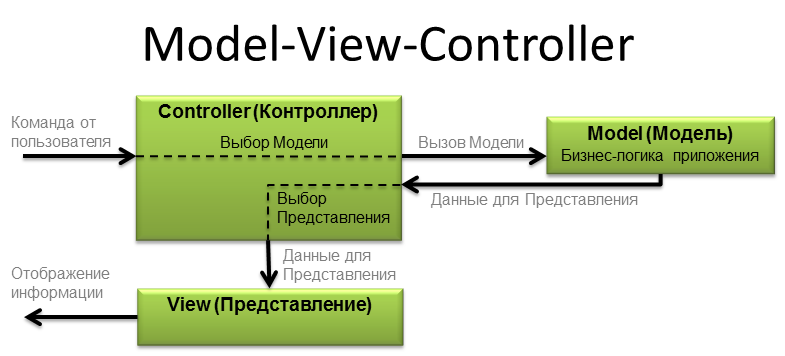
\includegraphics[scale=0.6]{mvc.png} 
	\caption{архитектурный шаблон Model-View-Controller}
	\label{fig:analysis:specification:language:mvc}
\end{figure}

Философия Rails включает два важных принципа:

\begin{itemize}
	\item Don't Repeat Yourself: DRY -- это принцип разработки ПО, который гласит, что "Каждый кусочек информации должен
	иметь единственное, неизбыточное, авторитетное представление в системе." Не пишите одну и ту же информацию снова и
	снова, код будет легче поддерживать, и он будет более расширяемым и менее ошибочным;
	\item Convention Over Configuration: у Rails есть мнения о наилучших способах делать множество вещей в веб-приложении,
	и по умолчанию выставлены эти соглашения, вместо того, чтобы заставлять вас по мелочам править многочисленные
	конфигурационные файлы~\cite{rails}.
\end{itemize}

По результатам обзора возможных платформ, представленных в пункте 1.1.2, было принято решение выбрать основной для
разработки платформу веб-приложений.

В качестве СУБД было принято решение использовать PostgreSQL - свободно распространяемую объектно-реляционную систему
управления базами данных, которая является наиболее развитой из открытых СУБД в мире и являющаяся реальной
альтернативой коммерческим базам данных.

Надежность PostgreSQL является проверенным и доказанным фактом и обеспечивается следующими возможностями:

\begin{itemize}
	\item полное соответствие принципам ACID -- атомарность, непротиворечивость, изолированность, сохранность данных.
	Атомарность -- транзакция рассматривается как единая логическая единица, все ее изменения или сохраняются целиком,
	или полностью откатываются. Непротиворечивость -- транзакция переводит базу данных из одного непротиворечивого
	состояния (на момент старта транзакции) в другое непротиворечивое состояние (на момент завершения транзакции).
	Непротиворечивым считается состояние базы, когда выполняются все ограничения физической и логической целостности
	базы данных, при этом допускается нарушение ограничений целостности в течение транзакции, но на момент завершения все
	ограничения целостности, как физические, так и логические, должны быть соблюдены. Изолированность -- изменения данных
	при конкурентных транзакциях изолированы друг от друга на основе системы версионности.
	Сохранность данных -- PostgreSQL заботится о том, что результаты успешных транзакций гарантировано сохраняются на
	жесткий диск вне зависимости от сбоев аппаратуры;
	\item многоверсионность используется для поддержания согласованности данных в конкурентных условиях, в то время как в
	традиционных базах данных используются блокировки. многоверсионность означает, что каждая транзакция видит копию
	данных (версию базы данных) на время начала транзакции, несмотря на то, что состояние базы могло уже измениться;
	\item репликация также повышает надежность PostgreSQL;
	\item открытость кодов PostgreSQL означает их абсолютную доступность для любого, а либеральная BSD лицензия не
	накладывает никаких ограничений на использование кода.
\end{itemize}

Производительность PostgreSQL основывается на использовании индексов, интеллектуальном планировщике запросов,
тонкой системы блокировок, системе управления буферами памяти и кэширования, превосходной масштабируемости при
конкурентной работе~\cite{postgres}.

Сформулированные требования позволят осуществить успешное проектирование и разработку программного средства.
